\documentclass[UTF8]{ctexart}
\usepackage{boxedminipage}
\usepackage{float}
\usepackage{hyperref}
\usepackage{graphicx}
\usepackage{multirow}
\usepackage{array}
%================样式================
\usepackage[paperwidth=210mm,paperheight=297mm,top=25.4mm,bottom=12.7mm,left=12.7mm,right=12.7mm]{geometry}
\setlength{\headsep}{3mm}
%\usepackage{setspace}
%\setstretch{1}
\usepackage{enumitem}
\setenumerate[1]{partopsep=0mm,parsep=\parskip,topsep=0mm}
%================交叉引用================
\renewcommand{\figureautorefname}{图}
%================快捷,与Python程序无关================
\newcommand{\smalltitle}[1]{{\zihao{4}\bfseries{#1}}\\} 
%================页眉================
\usepackage{fancyhdr}
\usepackage{lastpage}
\pagestyle{fancy}
\renewcommand{\headrulewidth}{0.5pt}
%\renewcommand{\footrulewidth}{0pt}
\fancyhf{}
\setlength{\headheight}{10mm}
\chead{
\centering
{\zihao{3}\textbf{生产作业指导书}}
}
%================正文的环境设置================
\begin{document}
\zihao{5}
\centering
%================正文内容================
\begin{boxedminipage}{184.6mm}
\centering
\smalltitle{开班准备描述}
\begin{boxedminipage}[t]{99.84mm}
\begin{enumerate}
\item 劳保鞋、静电服、静电手套穿戴整齐。不穿戴手套不得触摸零件。
\item 产线清线,非工作物料隔离。
\end{enumerate}
\end{boxedminipage}
\hfill
\begin{boxedminipage}[t]{76.76mm}
\begin{figure}[H]
\parbox[t]{36.38mm}{
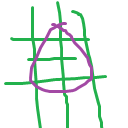
\includegraphics[width=36.38mm]{pic01}
\caption{}}
\hfill
\parbox[t]{36.38mm}{
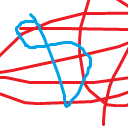
\includegraphics[width=36.38mm]{pic02}
\caption{}}
\end{figure}
\end{boxedminipage}
\end{boxedminipage}

\begin{boxedminipage}{184.6mm}
\centering
\smalltitle{设备开机描述}
\begin{boxedminipage}[t]{99.84mm}
\begin{enumerate}
\item 打开设备总电源,如图一。
\item 按下触摸屏下方的“设备上电”按钮,使其变为绿色,如图二。
\item 人员登录界面,选择“联机模式”,用户名输入“admin”,密码输入“admin”,点击“用户登录”,如图三。
\item 触摸屏点击上方的“目录页面”,随后在右侧选择“自动模式”如图四。
\item 此时触摸屏应当显示“没有报警”,即进入了正常生产模式。如若有报警,请按下触摸屏下方的“回初始位”按钮,设备回到原位后,该按钮应常亮黄色。随后转动“故障复位”旋钮,就能进入自动模式,如图五。
\end{enumerate}
\end{boxedminipage}
\hfill
\begin{boxedminipage}[t]{76.76mm}
图片2
\end{boxedminipage}
\end{boxedminipage}

\begin{boxedminipage}{184.6mm}
\centering
\setlength{\tabcolsep}{1mm}
\smalltitle{检查项目}
\begin{tabular}{|c|c|c|c|c|}
\firsthline
\multicolumn{2}{|c|}{\multirow{2}*{\parbox[c][][c]{86.3mm}{\centering \textbf{左上角大格}}}}&
\parbox[c][][s]{43.15mm}{\raggedright \smallskip \textbf{第3列上标题}\smallskip}&
\parbox[c][][s]{20.58mm}{\centering \smallskip \textbf{第4列上标题}\smallskip}&
\multirow{2}*{\parbox[c][][c]{20.58mm}{\centering \textbf{第5列标题}}}\\
\cline{3-4}
\multicolumn{2}{|c|}{}&
\parbox[c][][s]{43.15mm}{\raggedleft \smallskip \textbf{第3列下标题}\smallskip}&
\parbox[c][][s]{20.58mm}{\centering \smallskip \textbf{第4列下标题}\smallskip}&
\\
\hline
\parbox[c][][s]{9.29mm}{\centering \smallskip 1\smallskip}&
\parbox[c][][s]{77.01mm}{\raggedright \smallskip 扭杆压入力7-25KN\smallskip}&
\parbox[c][][s]{43.15mm}{\raggedright \smallskip 目视化点检\smallskip}&
\parbox[c][][s]{20.58mm}{\centering \smallskip 1件\smallskip}&
\parbox[c][][s]{20.58mm}{\centering \smallskip 首检\smallskip}\\
\hline
\parbox[c][][s]{9.29mm}{\centering \smallskip 2\smallskip}&
\parbox[c][][s]{77.01mm}{\raggedright \smallskip 扭杆压装距离112$\pm$1mm\smallskip}&
\parbox[c][][s]{43.15mm}{\raggedright \smallskip 高度尺\smallskip}&
\parbox[c][][s]{20.58mm}{\centering \smallskip 1件\smallskip}&
\parbox[c][][s]{20.58mm}{\centering \smallskip 首检\smallskip}\\
\hline
\parbox[c][][s]{9.29mm}{\centering \smallskip 3\smallskip}&
\parbox[c][][s]{77.01mm}{\raggedright \smallskip 自润滑衬套压入力0.15-1KN\smallskip}&
\parbox[c][][s]{43.15mm}{\raggedright \smallskip 目视化点检\smallskip}&
\parbox[c][][s]{20.58mm}{\centering \smallskip 1件\smallskip}&
\parbox[c][][s]{20.58mm}{\centering \smallskip 首检\smallskip}\\
\hline
\parbox[c][][s]{9.29mm}{\centering \smallskip 4\smallskip}&
\parbox[c][][s]{77.01mm}{\raggedright \smallskip 套入扭杆后油脂无溢出(0.02g$\ge$加脂量$\ge$0.1g)\smallskip}&
\parbox[c][][s]{43.15mm}{\raggedright \smallskip 电子秤\smallskip}&
\parbox[c][][s]{20.58mm}{\centering \smallskip 1件\smallskip}&
\parbox[c][][s]{20.58mm}{\centering \smallskip 首检\smallskip}\\
\hline
\parbox[c][][s]{9.29mm}{\centering \smallskip 5\smallskip}&
\parbox[c][][s]{77.01mm}{\raggedright \smallskip 自润滑衬套与输入轴压合距离6.5(+0.1/0)mm\smallskip}&
\parbox[c][][s]{43.15mm}{\raggedright \smallskip 游标卡尺\smallskip}&
\parbox[c][][s]{20.58mm}{\centering \smallskip 1件\smallskip}&
\parbox[c][][s]{20.58mm}{\centering \smallskip 首检\smallskip}\\
\hline
\parbox[c][][s]{9.29mm}{\centering \smallskip 6\smallskip}&
\parbox[c][][s]{77.01mm}{\raggedright \smallskip 扭杆上部圆跳动0.2\smallskip}&
\parbox[c][][s]{43.15mm}{\raggedright \smallskip ZN4350001\smallskip}&
\parbox[c][][s]{20.58mm}{\centering \smallskip 1件\smallskip}&
\parbox[c][][s]{20.58mm}{\centering \smallskip 首检\smallskip}\\
\hline
\parbox[c][][s]{9.29mm}{\centering \smallskip 7\smallskip}&
\parbox[c][][s]{77.01mm}{\raggedright \smallskip 扭杆靠近输出轴处圆跳动0.1\smallskip}&
\parbox[c][][s]{43.15mm}{\raggedright \smallskip ZN4350001\smallskip}&
\parbox[c][][s]{20.58mm}{\centering \smallskip 1件\smallskip}&
\parbox[c][][s]{20.58mm}{\centering \smallskip 首检\smallskip}\\
\lasthline
\end{tabular}

\end{boxedminipage}
\end{document}